\chapter{Processi e metodologie}
\label{cap:processi-metodologie}

\intro{In questo capitolo sono riassunti i processi e le metodologie che lo studente ha applicato durante lo sviluppo del progetto di stage.} 


\section{Ciclo di vita del software}
Il ciclo di vita del software è l'insieme delle attività e dei processi che tutti i membri coinvolti devono seguire per la buona riuscita del prodotto.
L'adozione di un modello di ciclo di vita è fondamentale per rispettare le scadenze, rimanere all'interno del \emph{budget} ed evitare conflitti all'interno e all'esterno del team.

\subsection{Filosofia Agile}
Per favorire la collaborazione l'azienda si affida alla filosofia \emph{agile}\footcite{site:agile} e in particolare al modello \emph{scrum} (Fig.~\ref{fig:schema-scrum}) che ha come unità fondamentale lo \emph{sprint} ossia un periodo di tempo breve (1 settimana) che viene utilizzato per sviluppare e testare nuove funzionalità; grazie a questi avanzamenti rapidi è possibile fornire codice flessibile e rapidamente adattabile alle nuove esigenze. 

\begin{figure}[!h] 
    \centering 
    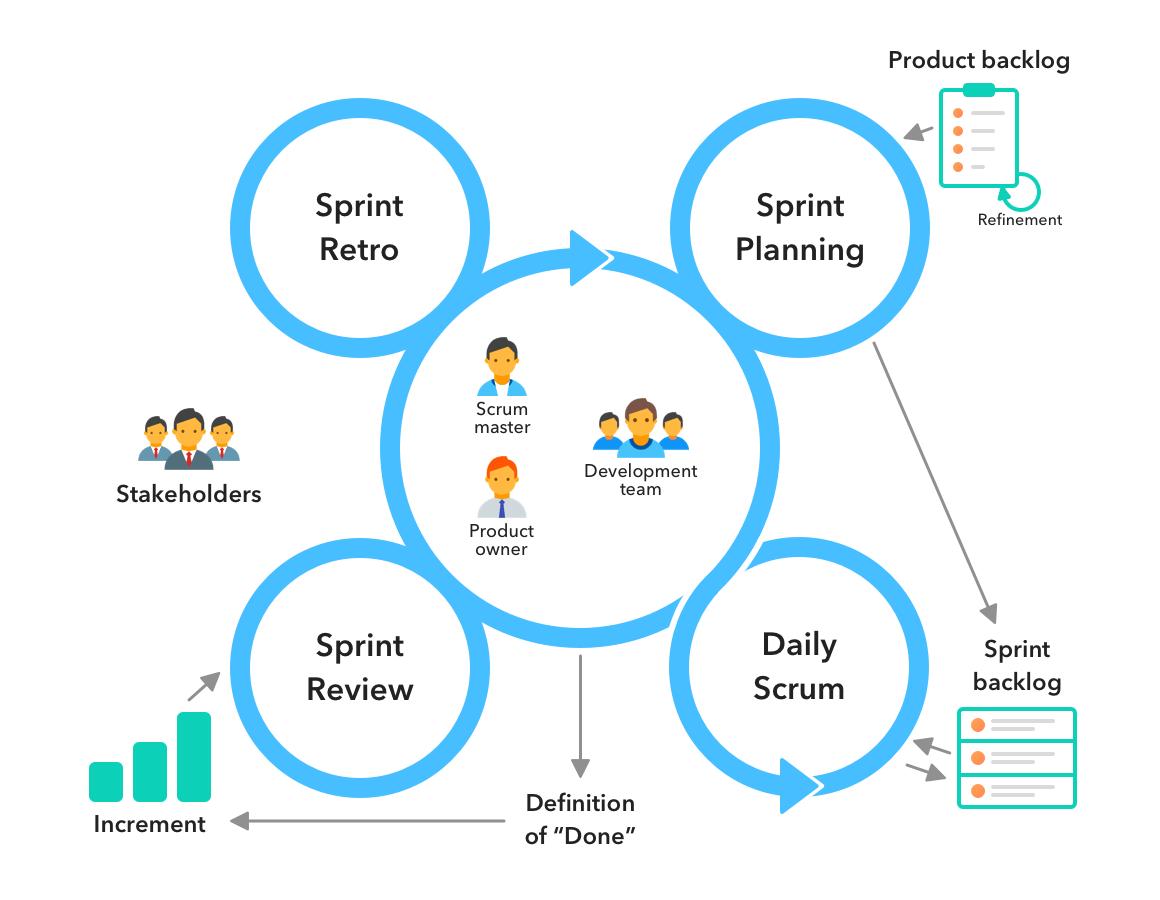
\includegraphics[width=0.6\columnwidth]{processi/scrum.png} 
    \caption{Schema del modello \emph{scrum}}
    \label{fig:schema-scrum}
  \end{figure}

\newpage

\subsection{Tecnologie di supporto}
\begin{itemize}
    \item Plane (Fig.~\ref{fig:logo-plane}): è un \emph{ITS (Issue Tracking System)} utilizzato per monitorare l'avanzamento del progetto e per assegnare a ciascun membro i compiti da effettuare; consente a tutte le parti coinvolte di avere una visione di insieme su quello che bisogna realizzare per portare a compimento lo sviluppo. In particolare è stato scelto perché altamente personalizzabile e per la sua natura \emph{\gls{open source}}\glsfirstoccur.
    
    \begin{figure}[!h] 
        \centering 
        
\includegraphics[width=0.4\columnwidth]{processi/plane-logo.png} 
        \caption{Logo di Plane}
        \label{fig:logo-plane}
      \end{figure}

    \item Telegram (Fig.~\ref{fig:logo-telegram}): è una piattaforma di messaggistica completa con molte funzionalità, viene sfruttata dall'azienda per coordinare i vari team di lavoro tramite l'ausilio di chat di gruppo. Fornisce inoltre molte funzionalità avanzate come \emph{\gls{bot}}\glsfirstoccur utili per i più svariati casi d'uso.
    
    \begin{figure}[!h] 
        \centering 
        
\includegraphics[width=0.4\columnwidth]{processi/telegram-logo.png} 
        \caption{Logo di Telegram}
        \label{fig:logo-telegram}
      \end{figure}
\end{itemize}

\newpage

\section{Gestione della configurazione}
La gestione della configurazione è il processo tramite il quale è possibile identificare, controllare e coordinare i vari componenti del software e le risorse a esso associate durante l'intero ciclo di vita del prodotto. Grazie a questo processo gli sviluppatori possono tenere traccia delle modifiche e gestire le varie versioni garantendo il funzionamento del prodotto nel tempo.



\subsection{Tecnologie di supporto}
Le tecnologie utilizzate per il versionamento del prodotto sono:
\begin{itemize}
    \item Git (Fig.~\ref{fig:logo-git}): è un \emph{DVCS (Distributed Version Controll System)} ampiamente diffuso che consente di gestire e monitorare i cambiamenti del codice e della documentazione. Questo strumento è fondamentale per avere una storia completa dello sviluppo da poter sfruttare in caso di necessità. Il codice viene inserito all'interno di un \emph{repository}, ossia una cartella che contiene tutti i file relativi al progetto, dove è possibile salvare ogni cambiamento tramite \emph{commit}. Il \emph{commit} segnala ogni modifica e la data in cui viene attuata, è dunque sufficiente spostarsi tra i vari \emph{commit} per tornare a una versione più o meno aggiornata.  
    
    \begin{figure}[!h] 
        \centering 
        
\includegraphics[width=0.6\columnwidth]{processi/git-logo.png} 
        \caption{Logo di Git}
        \label{fig:logo-git}
      \end{figure}

    \item Gitea (Fig.~\ref{fig:logo-gitea}): è un servizio che supporta le \emph{repository} di Git, è simile a GitHub, Bitbucket e GitLab, ma ha il vantaggio di essere \emph{\gls{self hosted}}\glsfirstoccur. 
    Essendo tutti i \emph{repository} aziendali mantenuti sul server interno, le comunicazioni atte al versionamento hanno risposta molto rapida.

    \begin{figure}[!h] 
        \centering 
        
\includegraphics[width=0.6\columnwidth]{processi/gitea-logo.png} 
        \caption{Logo di Gitea}
        \label{fig:logo-gitea}
      \end{figure}
\end{itemize}

\subsubsection{Regole di branch e commit}
Per standardizzare l'utilizzo delle tecnologie di versionamento l'azienda adotta due convenzioni:
\begin{itemize}
    \item \textbf{Git Flow}\footcite{site:gitflow} (Fig.~\ref{fig:schema-gitflow}): è un modello di \emph{\gls{branching}}\glsfirstoccur ideato per avere un miglior controllo delle \emph{release}.
    \item \textbf{Conventional Commits}\footcite{site:commits}: è una specifica basata su regole, che consentono una facile lettura dei \emph{commit} sia da parte di utenti che da parte di strumenti automatici. 
\end{itemize}

\begin{figure}[!h] 
    \centering 
    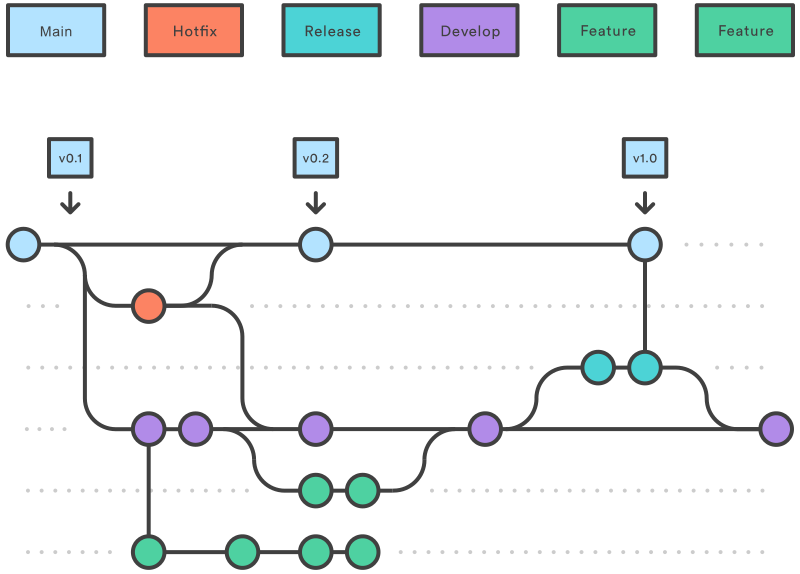
\includegraphics[width=0.9\columnwidth]{processi/gitflow.png} 
    \caption{Esempio di Git Flow}
    \label{fig:schema-gitflow}
  \end{figure}

  